% Created by tikzDevice version 0.12 on 2019-02-08 11:09:23
% !TEX encoding = UTF-8 Unicode
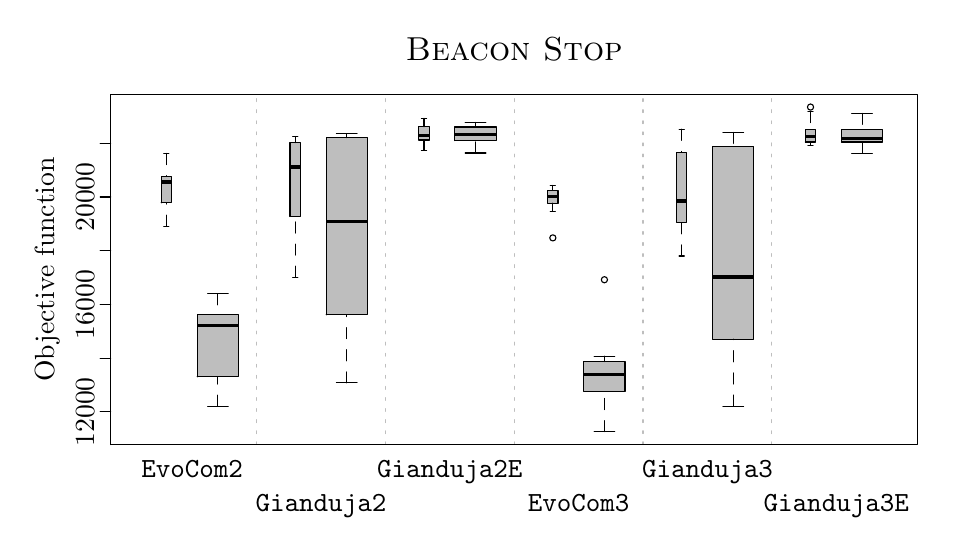
\begin{tikzpicture}[x=1pt,y=1pt]
\definecolor{fillColor}{RGB}{255,255,255}
\path[use as bounding box,fill=fillColor,fill opacity=0.00] (0,0) rectangle (325.21,180.67);
\begin{scope}
\path[clip] ( 30.00, 30.00) rectangle (321.61,156.67);
\definecolor{fillColor}{RGB}{190,190,190}

\path[fill=fillColor] ( 48.25,117.39) --
	( 51.97,117.39) --
	( 51.97,127.04) --
	( 48.25,127.04) --
	cycle;
\definecolor{drawColor}{RGB}{0,0,0}

\path[draw=drawColor,line width= 1.2pt,line join=round] ( 48.25,124.85) -- ( 51.97,124.85);

\path[draw=drawColor,line width= 0.4pt,dash pattern=on 4pt off 4pt ,line join=round,line cap=round] ( 50.11,108.94) -- ( 50.11,117.39);

\path[draw=drawColor,line width= 0.4pt,dash pattern=on 4pt off 4pt ,line join=round,line cap=round] ( 50.11,135.23) -- ( 50.11,127.04);

\path[draw=drawColor,line width= 0.4pt,line join=round,line cap=round] ( 49.18,108.94) -- ( 51.04,108.94);

\path[draw=drawColor,line width= 0.4pt,line join=round,line cap=round] ( 49.18,135.23) -- ( 51.04,135.23);

\path[draw=drawColor,line width= 0.4pt,line join=round,line cap=round] ( 48.25,117.39) --
	( 51.97,117.39) --
	( 51.97,127.04) --
	( 48.25,127.04) --
	( 48.25,117.39);

\path[fill=fillColor] ( 61.28, 54.52) --
	( 76.18, 54.52) --
	( 76.18, 77.09) --
	( 61.28, 77.09) --
	cycle;

\path[draw=drawColor,line width= 1.2pt,line join=round] ( 61.28, 73.09) -- ( 76.18, 73.09);

\path[draw=drawColor,line width= 0.4pt,dash pattern=on 4pt off 4pt ,line join=round,line cap=round] ( 68.73, 43.88) -- ( 68.73, 54.52);

\path[draw=drawColor,line width= 0.4pt,dash pattern=on 4pt off 4pt ,line join=round,line cap=round] ( 68.73, 84.49) -- ( 68.73, 77.09);

\path[draw=drawColor,line width= 0.4pt,line join=round,line cap=round] ( 65.01, 43.88) -- ( 72.46, 43.88);

\path[draw=drawColor,line width= 0.4pt,line join=round,line cap=round] ( 65.01, 84.49) -- ( 72.46, 84.49);

\path[draw=drawColor,line width= 0.4pt,line join=round,line cap=round] ( 61.28, 54.52) --
	( 76.18, 54.52) --
	( 76.18, 77.09) --
	( 61.28, 77.09) --
	( 61.28, 54.52);

\path[fill=fillColor] ( 94.80,112.41) --
	( 98.53,112.41) --
	( 98.53,139.15) --
	( 94.80,139.15) --
	cycle;

\path[draw=drawColor,line width= 1.2pt,line join=round] ( 94.80,130.30) -- ( 98.53,130.30);

\path[draw=drawColor,line width= 0.4pt,dash pattern=on 4pt off 4pt ,line join=round,line cap=round] ( 96.67, 90.47) -- ( 96.67,112.41);

\path[draw=drawColor,line width= 0.4pt,dash pattern=on 4pt off 4pt ,line join=round,line cap=round] ( 96.67,141.26) -- ( 96.67,139.15);

\path[draw=drawColor,line width= 0.4pt,line join=round,line cap=round] ( 95.73, 90.47) -- ( 97.60, 90.47);

\path[draw=drawColor,line width= 0.4pt,line join=round,line cap=round] ( 95.73,141.26) -- ( 97.60,141.26);

\path[draw=drawColor,line width= 0.4pt,line join=round,line cap=round] ( 94.80,112.41) --
	( 98.53,112.41) --
	( 98.53,139.15) --
	( 94.80,139.15) --
	( 94.80,112.41);

\path[fill=fillColor] (107.84, 76.91) --
	(122.74, 76.91) --
	(122.74,140.91) --
	(107.84,140.91) --
	cycle;

\path[draw=drawColor,line width= 1.2pt,line join=round] (107.84,110.58) -- (122.74,110.58);

\path[draw=drawColor,line width= 0.4pt,dash pattern=on 4pt off 4pt ,line join=round,line cap=round] (115.29, 52.30) -- (115.29, 76.91);

\path[draw=drawColor,line width= 0.4pt,dash pattern=on 4pt off 4pt ,line join=round,line cap=round] (115.29,142.30) -- (115.29,140.91);

\path[draw=drawColor,line width= 0.4pt,line join=round,line cap=round] (111.56, 52.30) -- (119.01, 52.30);

\path[draw=drawColor,line width= 0.4pt,line join=round,line cap=round] (111.56,142.30) -- (119.01,142.30);

\path[draw=drawColor,line width= 0.4pt,line join=round,line cap=round] (107.84, 76.91) --
	(122.74, 76.91) --
	(122.74,140.91) --
	(107.84,140.91) --
	(107.84, 76.91);

\path[fill=fillColor] (141.36,140.06) --
	(145.08,140.06) --
	(145.08,144.90) --
	(141.36,144.90) --
	cycle;

\path[draw=drawColor,line width= 1.2pt,line join=round] (141.36,141.70) -- (145.08,141.70);

\path[draw=drawColor,line width= 0.4pt,dash pattern=on 4pt off 4pt ,line join=round,line cap=round] (143.22,136.31) -- (143.22,140.06);

\path[draw=drawColor,line width= 0.4pt,dash pattern=on 4pt off 4pt ,line join=round,line cap=round] (143.22,147.90) -- (143.22,144.90);

\path[draw=drawColor,line width= 0.4pt,line join=round,line cap=round] (142.29,136.31) -- (144.15,136.31);

\path[draw=drawColor,line width= 0.4pt,line join=round,line cap=round] (142.29,147.90) -- (144.15,147.90);

\path[draw=drawColor,line width= 0.4pt,line join=round,line cap=round] (141.36,140.06) --
	(145.08,140.06) --
	(145.08,144.90) --
	(141.36,144.90) --
	(141.36,140.06);

\path[fill=fillColor] (154.39,139.90) --
	(169.29,139.90) --
	(169.29,144.76) --
	(154.39,144.76) --
	cycle;

\path[draw=drawColor,line width= 1.2pt,line join=round] (154.39,141.95) -- (169.29,141.95);

\path[draw=drawColor,line width= 0.4pt,dash pattern=on 4pt off 4pt ,line join=round,line cap=round] (161.84,135.38) -- (161.84,139.90);

\path[draw=drawColor,line width= 0.4pt,dash pattern=on 4pt off 4pt ,line join=round,line cap=round] (161.84,146.43) -- (161.84,144.76);

\path[draw=drawColor,line width= 0.4pt,line join=round,line cap=round] (158.12,135.38) -- (165.57,135.38);

\path[draw=drawColor,line width= 0.4pt,line join=round,line cap=round] (158.12,146.43) -- (165.57,146.43);

\path[draw=drawColor,line width= 0.4pt,line join=round,line cap=round] (154.39,139.90) --
	(169.29,139.90) --
	(169.29,144.76) --
	(154.39,144.76) --
	(154.39,139.90);

\path[fill=fillColor] (187.91,117.28) --
	(191.64,117.28) --
	(191.64,121.88) --
	(187.91,121.88) --
	cycle;

\path[draw=drawColor,line width= 1.2pt,line join=round] (187.91,119.59) -- (191.64,119.59);

\path[draw=drawColor,line width= 0.4pt,dash pattern=on 4pt off 4pt ,line join=round,line cap=round] (189.77,114.36) -- (189.77,117.28);

\path[draw=drawColor,line width= 0.4pt,dash pattern=on 4pt off 4pt ,line join=round,line cap=round] (189.77,123.70) -- (189.77,121.88);

\path[draw=drawColor,line width= 0.4pt,line join=round,line cap=round] (188.84,114.36) -- (190.70,114.36);

\path[draw=drawColor,line width= 0.4pt,line join=round,line cap=round] (188.84,123.70) -- (190.70,123.70);

\path[draw=drawColor,line width= 0.4pt,line join=round,line cap=round] (187.91,117.28) --
	(191.64,117.28) --
	(191.64,121.88) --
	(187.91,121.88) --
	(187.91,117.28);

\path[draw=drawColor,line width= 0.4pt,line join=round,line cap=round] (189.77,104.71) circle (  1.12);

\path[fill=fillColor] (200.95, 49.26) --
	(215.84, 49.26) --
	(215.84, 59.97) --
	(200.95, 59.97) --
	cycle;

\path[draw=drawColor,line width= 1.2pt,line join=round] (200.95, 55.28) -- (215.84, 55.28);

\path[draw=drawColor,line width= 0.4pt,dash pattern=on 4pt off 4pt ,line join=round,line cap=round] (208.40, 34.69) -- (208.40, 49.26);

\path[draw=drawColor,line width= 0.4pt,dash pattern=on 4pt off 4pt ,line join=round,line cap=round] (208.40, 61.97) -- (208.40, 59.97);

\path[draw=drawColor,line width= 0.4pt,line join=round,line cap=round] (204.67, 34.69) -- (212.12, 34.69);

\path[draw=drawColor,line width= 0.4pt,line join=round,line cap=round] (204.67, 61.97) -- (212.12, 61.97);

\path[draw=drawColor,line width= 0.4pt,line join=round,line cap=round] (200.95, 49.26) --
	(215.84, 49.26) --
	(215.84, 59.97) --
	(200.95, 59.97) --
	(200.95, 49.26);

\path[draw=drawColor,line width= 0.4pt,line join=round,line cap=round] (208.40, 89.59) circle (  1.12);

\path[fill=fillColor] (234.47,110.35) --
	(238.19,110.35) --
	(238.19,135.60) --
	(234.47,135.60) --
	cycle;

\path[draw=drawColor,line width= 1.2pt,line join=round] (234.47,118.09) -- (238.19,118.09);

\path[draw=drawColor,line width= 0.4pt,dash pattern=on 4pt off 4pt ,line join=round,line cap=round] (236.33, 98.17) -- (236.33,110.35);

\path[draw=drawColor,line width= 0.4pt,dash pattern=on 4pt off 4pt ,line join=round,line cap=round] (236.33,143.97) -- (236.33,135.60);

\path[draw=drawColor,line width= 0.4pt,line join=round,line cap=round] (235.40, 98.17) -- (237.26, 98.17);

\path[draw=drawColor,line width= 0.4pt,line join=round,line cap=round] (235.40,143.97) -- (237.26,143.97);

\path[draw=drawColor,line width= 0.4pt,line join=round,line cap=round] (234.47,110.35) --
	(238.19,110.35) --
	(238.19,135.60) --
	(234.47,135.60) --
	(234.47,110.35);

\path[fill=fillColor] (247.50, 68.09) --
	(262.40, 68.09) --
	(262.40,137.78) --
	(247.50,137.78) --
	cycle;

\path[draw=drawColor,line width= 1.2pt,line join=round] (247.50, 90.60) -- (262.40, 90.60);

\path[draw=drawColor,line width= 0.4pt,dash pattern=on 4pt off 4pt ,line join=round,line cap=round] (254.95, 43.92) -- (254.95, 68.09);

\path[draw=drawColor,line width= 0.4pt,dash pattern=on 4pt off 4pt ,line join=round,line cap=round] (254.95,142.83) -- (254.95,137.78);

\path[draw=drawColor,line width= 0.4pt,line join=round,line cap=round] (251.23, 43.92) -- (258.67, 43.92);

\path[draw=drawColor,line width= 0.4pt,line join=round,line cap=round] (251.23,142.83) -- (258.67,142.83);

\path[draw=drawColor,line width= 0.4pt,line join=round,line cap=round] (247.50, 68.09) --
	(262.40, 68.09) --
	(262.40,137.78) --
	(247.50,137.78) --
	(247.50, 68.09);

\path[fill=fillColor] (281.02,139.35) --
	(284.74,139.35) --
	(284.74,143.92) --
	(281.02,143.92) --
	cycle;

\path[draw=drawColor,line width= 1.2pt,line join=round] (281.02,141.34) -- (284.74,141.34);

\path[draw=drawColor,line width= 0.4pt,dash pattern=on 4pt off 4pt ,line join=round,line cap=round] (282.88,138.24) -- (282.88,139.35);

\path[draw=drawColor,line width= 0.4pt,dash pattern=on 4pt off 4pt ,line join=round,line cap=round] (282.88,150.36) -- (282.88,143.92);

\path[draw=drawColor,line width= 0.4pt,line join=round,line cap=round] (281.95,138.24) -- (283.81,138.24);

\path[draw=drawColor,line width= 0.4pt,line join=round,line cap=round] (281.95,150.36) -- (283.81,150.36);

\path[draw=drawColor,line width= 0.4pt,line join=round,line cap=round] (281.02,139.35) --
	(284.74,139.35) --
	(284.74,143.92) --
	(281.02,143.92) --
	(281.02,139.35);

\path[draw=drawColor,line width= 0.4pt,line join=round,line cap=round] (282.88,151.98) circle (  1.12);

\path[fill=fillColor] (294.05,139.37) --
	(308.95,139.37) --
	(308.95,143.77) --
	(294.05,143.77) --
	cycle;

\path[draw=drawColor,line width= 1.2pt,line join=round] (294.05,140.70) -- (308.95,140.70);

\path[draw=drawColor,line width= 0.4pt,dash pattern=on 4pt off 4pt ,line join=round,line cap=round] (301.50,135.34) -- (301.50,139.37);

\path[draw=drawColor,line width= 0.4pt,dash pattern=on 4pt off 4pt ,line join=round,line cap=round] (301.50,149.71) -- (301.50,143.77);

\path[draw=drawColor,line width= 0.4pt,line join=round,line cap=round] (297.78,135.34) -- (305.23,135.34);

\path[draw=drawColor,line width= 0.4pt,line join=round,line cap=round] (297.78,149.71) -- (305.23,149.71);

\path[draw=drawColor,line width= 0.4pt,line join=round,line cap=round] (294.05,139.37) --
	(308.95,139.37) --
	(308.95,143.77) --
	(294.05,143.77) --
	(294.05,139.37);
\definecolor{drawColor}{RGB}{190,190,190}

\path[draw=drawColor,line width= 0.4pt,dash pattern=on 1pt off 3pt ,line join=round,line cap=round] ( 82.70, 30.00) -- ( 82.70,156.67);

\path[draw=drawColor,line width= 0.4pt,dash pattern=on 1pt off 3pt ,line join=round,line cap=round] (129.25, 30.00) -- (129.25,156.67);

\path[draw=drawColor,line width= 0.4pt,dash pattern=on 1pt off 3pt ,line join=round,line cap=round] (175.81, 30.00) -- (175.81,156.67);

\path[draw=drawColor,line width= 0.4pt,dash pattern=on 1pt off 3pt ,line join=round,line cap=round] (222.36, 30.00) -- (222.36,156.67);

\path[draw=drawColor,line width= 0.4pt,dash pattern=on 1pt off 3pt ,line join=round,line cap=round] (268.92, 30.00) -- (268.92,156.67);
\end{scope}
\begin{scope}
\path[clip] (  0.00,  0.00) rectangle (325.21,180.67);
\definecolor{drawColor}{RGB}{0,0,0}

\node[text=drawColor,anchor=base,inner sep=0pt, outer sep=0pt, scale=  1.00] at ( 59.42, 18.00) {\texttt{EvoCom2}};

\node[text=drawColor,anchor=base,inner sep=0pt, outer sep=0pt, scale=  1.00] at (152.53, 18.00) {\texttt{Gianduja2E}};

\node[text=drawColor,anchor=base,inner sep=0pt, outer sep=0pt, scale=  1.00] at (245.64, 18.00) {\texttt{Gianduja3}};

\node[text=drawColor,anchor=base,inner sep=0pt, outer sep=0pt, scale=  1.00] at (105.98,  6.00) {\texttt{Gianduja2}};

\node[text=drawColor,anchor=base,inner sep=0pt, outer sep=0pt, scale=  1.00] at (199.08,  6.00) {\texttt{EvoCom3}};

\node[text=drawColor,anchor=base,inner sep=0pt, outer sep=0pt, scale=  1.00] at (292.19,  6.00) {\texttt{Gianduja3E}};
\end{scope}
\begin{scope}
\path[clip] (  0.00,  0.00) rectangle (325.21,180.67);
\definecolor{drawColor}{RGB}{0,0,0}

\node[text=drawColor,anchor=base,inner sep=0pt, outer sep=0pt, scale=  1.20] at (175.81,168.67) {\textsc{Beacon Stop}};

\node[text=drawColor,rotate= 90.00,anchor=base,inner sep=0pt, outer sep=0pt, scale=  1.00] at (  9.60, 93.34) {Objective function};
\end{scope}
\begin{scope}
\path[clip] (  0.00,  0.00) rectangle (325.21,180.67);
\definecolor{drawColor}{RGB}{0,0,0}

\path[draw=drawColor,line width= 0.4pt,line join=round,line cap=round] ( 30.00, 41.83) -- ( 30.00,138.88);

\path[draw=drawColor,line width= 0.4pt,line join=round,line cap=round] ( 30.00, 41.83) -- ( 26.20, 41.83);

\path[draw=drawColor,line width= 0.4pt,line join=round,line cap=round] ( 30.00, 61.24) -- ( 26.20, 61.24);

\path[draw=drawColor,line width= 0.4pt,line join=round,line cap=round] ( 30.00, 80.65) -- ( 26.20, 80.65);

\path[draw=drawColor,line width= 0.4pt,line join=round,line cap=round] ( 30.00,100.06) -- ( 26.20,100.06);

\path[draw=drawColor,line width= 0.4pt,line join=round,line cap=round] ( 30.00,119.47) -- ( 26.20,119.47);

\path[draw=drawColor,line width= 0.4pt,line join=round,line cap=round] ( 30.00,138.88) -- ( 26.20,138.88);

\node[text=drawColor,rotate= 90.00,anchor=base,inner sep=0pt, outer sep=0pt, scale=  1.00] at ( 24.00, 41.83) {12000};

\node[text=drawColor,rotate= 90.00,anchor=base,inner sep=0pt, outer sep=0pt, scale=  1.00] at ( 24.00, 80.65) {16000};

\node[text=drawColor,rotate= 90.00,anchor=base,inner sep=0pt, outer sep=0pt, scale=  1.00] at ( 24.00,119.47) {20000};

\path[draw=drawColor,line width= 0.4pt,line join=round,line cap=round] ( 30.00, 30.00) --
	(321.61, 30.00) --
	(321.61,156.67) --
	( 30.00,156.67) --
	( 30.00, 30.00);
\end{scope}
\end{tikzpicture}
